%!TEX root = ../cwqo.tex
\section{Bad Patterns In Tree Decompositions}
\label{sec:bad-patterns}

In this section, we will prove the main theorem of this paper, which provides
an effective algorithm to decide if a class of graphs of bounded clique-width
is well-quasi-ordered. 

\begin{theorem}[restate=effective-image:thm,label={effective-image:thm}]
    \label{effective-image:thm}
    Let $I$ be an $\MSO$ interpretation
    from finite trees to undirected graphs.
    There exists a computable $k \in \Nat$
    such that $\image{I}$
    is $k$-well-quasi-ordered
    if and only if 
    $\image{I}$ is wqo-well-quasi-ordered.
    These properties are furthermore decidable.
\end{theorem}

From this theorem, we immediately provide a positive answer to
\cref{pouzet2:conj} for classes of graphs of \kl{bounded clique-width}.

\begin{corollary}
    \label{effective-image:cor}
    A class of graphs $\Cls$ of \kl{bounded clique width} 
    is \kl{labelled-well-quasi-ordered}
    if and only if it is \kl{wqo-well-quasi-ordered}.
\end{corollary}
\begin{proof}
    Consider a class $\Cls$ of graphs having bounded clique width.
    There is an interpretation from trees to a superset of this class $\Cls$.
    Because $\Cls$ is \kl{labelled-well-quasi-ordered}, the class of images
    can be described using finitely many forbidden patterns,
    and we can assume that we do not take subsets.
    As a consequence, we can assume that there exists a $\varphi$
    such that $\Cls \subseteq \varphi(\Trees{\Sigma}) \subseteq \dwset{\Cls}$.
    Now, because $\Cls$ is \kl{labelled-well-quasi-ordered}, we can assume that
    $\dwset{\Cls}$ is \kl{labelled-well-quasi-ordered} as well.
    This proves that $\varphi(\Trees{\Sigma})$ is \kl{labelled-well-quasi-ordered},
    hence \kl{wqo-well-quasi-ordered},
    and as a consequence so is $\Cls$.
\end{proof}

Before proving \cref{effective-image:thm}, let us focus our attention on
\intro{simple interpretations}, i.e., those that are defined solely by a
formula $\varphi_E(x,y)$.
This is not a restriction, as the following lemma
shows.

\begin{lemma}
    \label{simple-interpretation:lem}
    Let $I$ be an $\MSO$ interpretation from finite trees to undirected graphs.
    There exists a (computable) simple interpretation $I'$ such that
    for all $k \geq 1$,
    $\image{I}$ is \kl{$k$-well-quasi-ordered} if and only if
    $\image{I'}$ is \kl{$k$-well-quasi-ordered}.
\end{lemma}
\begin{proof}
\end{proof}

\subsection{From Interpretation to Monoids}

\AP In this section, we will use standard construction from automata theory,
and especially the equivalence between $\MSO$-formulas on trees and bottom-up
deterministic tree-automata. We refer to the book on Tree Automata Techniques
and Applications for a comprehensive overview of this topic \cite{TATA08}. It
follows from standard arguments that to a formula $\varphi(x,y)$ over binary
trees labelled using letters in $\Sigma$ one can associate a monoid $M$ and a
morphism $\mu \colon \Sigma^* \to M$ such that for any tree $T$ and any pair of
leaves $x,y$ in $T$, whether $T \models \varphi(x,y)$ is entirely determined by
the values of $\mu(T[z \colon x])$, $\mu(T[z \colon y])$ and $\mu(T[\treeRoot
\colon z])$ where $z = \lca(x,y)$ is the \kl{ least common ancestor} of $x$ and
$y$.
As a consequence,
one can collect in a subset $P \subseteq M^3$ all the triples $(a,b,c)$ such
that this triple corresponds to a satisfying assignment of the formula
$\varphi(x,y)$.
This is illustrated in \cref{interpretation-to-monoid:fig}. 

\AP In order to simplify notations and better distinguish between the labels of
the nodes (in a finite alphabet $\Sigma$) and their corresponding elements in
the monoid $M$, we will label the \emph{edges} of the trees by the elements of
$M$, having a special treatment for the root of the tree. Given two nodes $x
\treelt[T] y$ in a tree $T$, we will write $\tlbl{T}{x}{y}$ for the product of
the edge labels on the path from $x$ to $y$ in $T$.  Furthermore, we assume for
the rest of the section that the monoid $M$ and the morphism $\mu$ are fixed,
together with the accepting part $P \subseteq M^3$. As a consequence, when we
refer to trees in this subsection, they have nodes labelled by $\Sigma$ and
edges labelled by $M$. Given such a tree $T$, we define $\treeSem{T}$ as the
graph obtained by considering leaves of $T$ as vertices, and placing an edge
between two leaves $x$ and $y$ if and only if $(\tlbl{T}{z}{x}, \tlbl{T}{z}{y},
\tlbl{T}{\treeRoot}{z}) \in P$ where $z = \lca(x,y)$.

\begin{figure}
    \centering
    \begin{tikzpicture}[
        leaf/.style={
            color=Prune
        },
        lca/.style={
            color=A1
        },
        edge/.style={
            color=A2
        },
        root/.style={
            color=Prune
        },
        gedge/.style={
            color=A4
        },
        ]
        \node[root] (root) at (0,1) {$\treeRoot$};
        \node[leaf] (x) at (-1,-1) {$x$};
        \node[leaf] (y) at (1,-1) {$y$};
        \node[lca] (lca) at (0,0) {$\lca(x,y)$};
        \coordinate (tl) at ($(x.south west)+(-0.2,0)$);
        \coordinate (tr) at ($(y.south east)+(0.2,0) $);
        \coordinate (t)  at ($(root.north)+(0, 1)$);
        \draw[edge,->] (root) to node[midway, left]        {$a$}  (lca);
        \draw[edge,->] (lca)  to node[midway, above  left] {$b$} (x);
        \draw[edge,->] (lca)  to node[midway, above right] {$c$} (y);
        \draw (tl) -- (tr) -- (t) -- cycle;

        \node (maps-to) at (3,0) {$\mapsto$};

        \begin{scope}[xshift=4cm]
            \node[leaf] (nx) at (0,0) {$x$};
            \node[leaf] (ny) at (5,0) {$y$};
            \draw[gedge] (nx) to node[midway, above] {$(a,b,c) \in P$?} (ny);
        \end{scope}
    \end{tikzpicture}
    \caption{The interpretation of a tree using a monoid and an accepting part.}
    \label{interpretation-to-monoid:fig}
\end{figure}

The main idea of using monoids to encode the truth value of $\varphi(x,y)$ is
that one can then use a suitable notion of tree embeddings makes the
interpretation from trees to graphs \emph{monotone}.

\begin{definition}
    \label{composition-ordering:def}
    Let $T_1$ and $T_2$ be two trees. 
    A map $h \colon T_1 \to T_2$ is an \intro{compositional tree embedding}
    if it is a \kl{tree embedding} and
    for all pairs of nodes $x \treelt[T_1] y$ in $T_1$, 
    we have $\tlbl{T_1}{x}{y} = \tlbl{T_2}{h(x)}{h(y)}$.
\end{definition}

\begin{lemma}
    \label{composition-ordering:lem}
    Let $T_1$ and $T_2$ be two trees such that
    $h \colon T_1 \to T_2$ is a \kl{compositional tree embedding}.
    Then, $h \colon \treeSem{T_1} \to \treeSem{T_2}$
    is a \kl{labelled graph embedding}.
\end{lemma}
\begin{proof}
\end{proof}

\AP As a consequence, it is sufficient to understand when the \kl{composition
ordering} on trees is well-quasi-ordered to understand when the \kl{labelled
graph embedding} is well-quasi-ordered. Historically, this was (although not
explicitly) the approach taken by \cite{DRT10}. Unfortunately, the composition
ordering on trees is more often than not way more strict than the \kl{induced
subgraph} ordering. It was already observed that the composition ordering on
trees is \kl{well-quasi-ordered} if and only if \emph{for every} $Q \subseteq
M^3$, the class of graphs obtained from trees by considering only the triples
in $Q$ is \kl{labelled-well-quasi-ordered} \cite{LOPEZ24}. To understand what
happens for a precise choice of $Q$, we need to have a finer understanding of
the way trees can be decomposed.




\begin{figure}
    \centering
    \todo[inline]{Draw the composition ordering on trees}
    \caption{The composition ordering on trees}
    \label{composition-ordering:fig}
\end{figure}

\subsection{Forward Ramseyan Splits and Bad Branches}

\def\t{\aTree} \AP The crucial combinatorial ingredient to understand how to
decompose further the trees will come from an adaptation of the classical Simon
Factorisation Theorem for semigroups \cite{SIMO90}, adapted to trees by
Colcombet \cite{COLC07}. A \intro{split of height $N$} of a tree $\t$ is a
mapping $\spt$ from the nodes of $T$ to $\set{1, \dots, N}$. Given a split
$\spt$ and two nodes $x \treelt[\t] y$, we define $\spt(x \colon y)$ to be the
minimal value of $\spt(z)$ for $x \treelt[\t] z \treelt[\t] y$, and $\infty$
otherwise. Two elements $x \treelt[\t] y$ such that $\spt(x) = \spt(y) = k$ are
\intro{$k$-neighbours} if $\spt(x \colon y) \geq k$.

\AP A split $\spt$ is \intro{forward Ramseyan} if for every $k \in \set{1,
\dots, N}$ and every $x, y, x', y'$ in the same class of \kl{$k$-neighbourhood}
with $x \treelt[\t] y$ and $x' \treelt[\t] y'$, we have:
\begin{equation}
    \label{fake-idempotent:eq} 
    \tlbl{\t}{x}{y} = \tlbl{\t}{x}{y} \cdot \tlbl{\t}{x'}{y'} \quad .
\end{equation} 

\AP
In particular, $\tlbl{\t}{x}{y}$ is an \kl{idempotent}, since $\tlbl{\t}{x}{y}
\cdot \tlbl{\t}{x}{y} = \tlbl{\t}{x}{y}$, but $\tlbl{\t}{x}{y}$ and
$\tlbl{\t}{x'}{y'}$ may be different \kl{idempotents}. 

\AP Let us illustrate how one can use \kl{forward Ramseyan splits} to compute
efficiently the value of $\tlbl{\t}{x}{y}$ for any pair of nodes $x \treelt[\t]
y$. We are going to paraphrase the actual content of \cite[Lemma 3]{COLC07},
using the drawing of \cref{fast-computation:fig} to explain the idea. We claim
that to compute the value of $\tlbl{\t}{x}{y}$, one can restrict the
computation to \emph{few} specific segments of the path from $x$ to $y$ with a
\emph{strictly larger} value of $\spt$. The reason is that whenever $x$ and $y$
are separated by many nodes $z$ such that $\spt(z) = \spt(x:y)$, one can
essentially ignore all but the first and last such nodes to speed up
computation. This of course can be applied recursively leading to a fast (and
first-order definable, provided the split $\spt$ is known) algorithm to compute
the value of $\tlbl{\t}{x}{y}$.

\begin{figure}
    \centering
    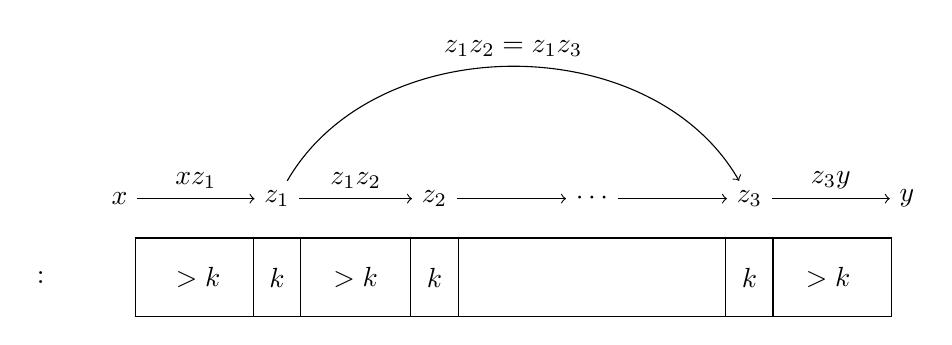
\begin{tikzpicture}
        \node (s) at (-1,-1) {$\spt \colon $};
        \node (x) at (0,0) {$x$};
        \node (z1) at (2,0) {$z_1$};
        \node (z2) at (4,0) {$z_2$};
        \node (z3) at (6,0) {$\cdots$};
        \node (z4) at (8,0) {$z_3$};
        \node (y) at (10,0) {$y$};

        \node[below of=z1] {$k$};
        \node[below of=z2] {$k$};
        \node[below of=z4] {$k$};
        \node (xz1) at (1,-1) {$> k$};
        \node (z1z2) at (3,-1) {$> k$};
        \node (z4y) at (9,-1) {$> k$};

        \draw (0.2,-0.5) rectangle (9.8,-1.5);
        \draw (1.7,-0.5) -- (1.7, -1.5);
        \draw (2.3,-0.5) -- (2.3, -1.5);

        \draw (3.7,-0.5) -- (3.7, -1.5);
        \draw (4.3,-0.5) -- (4.3, -1.5);

        \draw (7.7,-0.5) -- (7.7, -1.5);
        \draw (8.3,-0.5) -- (8.3, -1.5);


        \draw[->] (x) -- 
        node[midway, above] {$\tlbl{\t}{x}{z_1}$}
        (z1);
        \draw[->] (z1) --
        node[midway, above] {$\tlbl{\t}{z_1}{z_2}$}
        (z2);
        \draw[->] (z2) -- (z3);
        \draw[->] (z3) -- (z4);
        \draw[->] (z4) -- 
        node[midway, above] {$\tlbl{\t}{z_3}{y}$}
        (y);
        \draw[->] (z1) to[bend left=60] 
        node[midway, above] {$\tlbl{\t}{z_1}{z_2} = \tlbl{\t}{z_1}{z_3}$}
        (z4);

    \end{tikzpicture}
    \caption{Fast computation of the value $\tlbl{\t}{x}{y}$
        provided a forward Ramseyan split.}
    \label{fast-computation:fig}
\end{figure}

\AP The main theorem of \cite{COLC07} is that for every finite monoid $M$,
there exists a finite depth $N$ such that for every tree $T$ labelled using
$M$, there exists a forward Ramseyan split of height $N$ for $T$. We can
therefore assume that our trees are always equipped with a forward Ramseyan
split of height $N$.

\AP One can define a notion of embedding between two trees equipped with their
respective \kl{forward Ramseyan splits}. Given two trees $\t_1$ and $\t_2$ with
their respective splits $\spt_1$ and $\spt_2$, a map $h \colon \t_1 \to \t_2$
is a \intro{gap embedding} if it is a \kl{tree embedding} and for all
\kl{$k$-neighbouring} nodes $x \treelt[\t_1] y$ in $\t_1$, $h(x) \treelt[\t_2]
h(y)$ are \kl{$k$-neighbouring} nodes in $\t_2$. Trees equipped with
\kl{forward Ramseyan splits} form a \kl{well-quasi-ordered} set with respect to
the \kl{gap embedding} relation \cite{DERSHOWITZ200380}.

\AP Let us introduce a notion of dependency between nodes that will allow us to
explain how the \kl{gap embedding} relation preserves \emph{some} of the monoid
products in the trees. A node $x$ is \intro{independent at level $k$} from a
node $y$, written $x \bot_k y$ if $x$ is \kl{independent at level $k+1$} and
$\spt(x:y) \geq k+1$ or if there exist three nodes $z_1, z_2, z_3$ such that
$x \treelt[\t] z_1 \treelt[\t] z_2 \treeleq[\t] z_3 \treelt[\t] y$ such that
$\spt(z_1) = \spt(z_2) = \spt(z_3) = k$, $x \bot_{k+1} z_1$, $z_1 \bot_{k+1}
z_2$, and $z_3 \bot_{k+1} y$. If $k = N+1$, then $x \bot_{N+1} y$ if $x$ is the
immediate ancestor of $y$ in the tree.

\begin{lemma}
    Let $h \colon (T, \spt) \to (T', \spt')$ be a \kl{gap embedding} between two
    trees equipped with \kl{forward Ramseyan splits}. Then, for all $x \bot_k y$
    in $T$, we have $\tlbl{T}{x}{y} = \tlbl{T'}{h(x)}{h(y)}$.
\end{lemma}
\begin{proof}
    By immediate induction on $\spt(x:y)$.
\end{proof}

\AP Therefore, the main combinatorial obstacle to understanding whether or not
a class is \kl{labelled-well-quasi-ordered} is to understand the behaviour of
pairs of nodes $x$ and $y$ that are \kl{dependent}. This is the motivation
for the following construction that studies the behaviour of
consecutive \kl{$k$-neighbourhoods} in a tree.

\begin{definition}
    \label{ramseyan-branch:def}
    Let $T$ be a tree and $\spt$ be a \kl{forward Ramseyan split} of height $N$.
    A \intro{bough of level $k$} in $T$ is an infix of a branch of $T$
    satisfying:
    \begin{enumerate}
        \item Its maximal and minimal elements have level $k$
        \item All elements of the bough have level greater or equal to $k$
    \end{enumerate}
    The \intro{size of a bough} is the number of elements of depth $k$
    in the \kl{bough}.
\end{definition}

\AP Let $B$ be a \kl{bough of level $k$} in $T$. Given two nodes $b_1$ and
$b_2$ in $B$ such that $\spt(b_1) = \spt(b_2) = k$, we define the $T_{b_1:b_2}$
as the set of nodes $x$ in $T$ such that $b_1 \treeleq x$ and $\neg (b_2
\treeleq x)$. For every leaf $x \in T_{b_0: b_n}$ where $n$ is the size of the
bough $B$, we define $\Bt(x)$ to be the least ancestor of $x$ that belongs to
$B$. Similarly, we define $\Bl(x)$ to be the least element of $B$ that is
greater or equal to $\Bt(x)$, and $\Br(x)$ to be the greatest element of $B$
that is less or equal to $\Bt(x)$. To every leaf $x$ of $B(T)$, we can
therefore associate a triple of values: $\BtL(x) \defined
\tlbl{\t}{\Bt(x)}{x}$, $\BlL(x) \defined \tlbl{\t}{\Bl(x)}{\Bt(x)}$, and
$\BrL(x) \defined \tlbl{\t}{\Bt(x)}{\Br(x)}$. We refer to
\cref{type-of-a-leaf-in-branch:fig} for an
illustration of the type of a leaf with respect to a given \kl{bough} $B$.
We also refer to \cref{partitionning-a-graph:fig} for an illustration of the
resulting partition of the tree $T$ with respect to a given \kl{bough} $B$.

\begin{figure}
    \centering
    \begin{tikzpicture}[
        branch/.style={
            color=Prune,
            inner sep=0pt,
            minimum size=4pt,
            fill,
            circle
        },
        inner/.style={
            color=A1,
            inner sep=0pt,
            minimum size=4pt,
            draw,
            circle
        },
        staredge/.style={
            color=A1,
            ->,
            dashed
        },
        root/.style={
            color=Prune,
        },
        leaf/.style={
            color=Prune,
        },
        monoid/.style={
            color=A2
        },
        ]
        % first draw the branch 
        \node[root]   (root) at (-2,0) {$\treeRoot$};
        \node[branch] (b0) at (0,0) {};
        \node[branch] (b1) at (4,0) {};
        \node[inner]  (t)  at (2,0) {};
        \node[leaf]   (x)  at (3.5,-2) {$x$};

        \node[above=0.1cm of b0] {$\Bl(x)$};
        \node[above=0.1cm of t]  {$\Bt(x)$};
        \node[above=0.1cm of b1] {$\Br(x)$};

        \draw[staredge] (root) -- (b0);
        \draw[staredge] (b0) -- node[monoid, midway, below] {$\BlL(x)$} (t);
        \draw[staredge] (t)  -- node[monoid, midway, below] {$\BrL(x)$} (b1);
        \draw[staredge] (b1) -- (5,0);

        \draw[staredge] (t)  -- node[monoid, midway, below left] {$\BtL(x)$} (x);
    \end{tikzpicture}
    \caption{The type of a leaf with respect to a given \kl{bough} $B$.}
    \label{type-of-a-leaf-in-branch:fig}
\end{figure}

\begin{figure}
    \centering
    \begin{tikzpicture}[
        localType/.style={
            color=C3,
            thick
        },
        branchProj/.style = {
            color=Prune,
            inner sep=0pt,
            minimum size=4pt,
            fill,
            circle
        },
        leaf/.style={
            color=Prune,
        },
        ]
        \draw (0,0) rectangle (8,2);
        \node (root) at (-2,2) {$\treeRoot$};
        \foreach \x in {0,1,2,3,4} {
            \coordinate (n\x) at ({ 2 * \x},0);
            \coordinate (pb\x) at ({ 2 * \x},2);
            \node[branchProj] (b\x) at (pb\x) {};
            \node (lb\x) at ({ 2 * \x},2.4) {$b_{\x}$};
            \draw (n\x) -- (b\x);
        }
        \draw[dashed,<-] (b0) -- (root);
        \draw[dashed] (b4) -- (9,2);
        \draw[dashed] (n4) -- (9,0);

        \foreach[count=\x] \y in {0,1,2,3} {
            \node (E\x) at ({ 2 * \x - 1},2.6) {$e_{\y}$};
            \draw[->,thick] (b\y) to[bend left=40] (b\x);
            \node (T\x) at ({ 2 * \x - 1},-0.6) {$T_{b_{\y}:b_{\x}}$};
        }
        
        \node (x) at (3,0.2)  {$x$};
        \node (y) at (7,0.2)  {$y$};
        \node[branchProj] (tx) at (3,2) {};
        \node[branchProj] (ty) at (7,2) {};

        \draw[localType, <-] (x)  -- 
        node[midway, left] {$\BtL(x)$} (tx);
        (tx);
        \draw[localType, ->] (tx) -- 
        node[midway, below] {$\BrL(x)$}
        (b2);
        \draw[localType, <-] (tx) -- 
        node[midway, below] {$\BlL(x)$}
        (b1);

        \draw[localType, <-] (y)  -- 
        node[midway, left] {$\BtL(y)$} 
        (ty);
        \draw[localType, ->] (ty) -- 
        node[midway, below] {$\BrL(y)$}
        (b4);
        \draw[localType, <-] (ty) --
        node[midway, below] {$\BlL(y)$}
        (b3);


    \end{tikzpicture}
    \caption{Partitionning a graph using a branch.}
    \label{partitionning-a-graph:fig}
\end{figure}

\AP
To compute the presence of an edge between two leaves $x$ and $y$
in $B(T)$, we only need to know their respective \kl{bough types}
the order in which they appear in the \kl{bough}, 
and whether or not there is an idempotent. \cref{partitionning-a-graph:fig}.

\begin{definition}
    \label{good-bough:def}
    Let $B$ be a \kl{bough} of level $k$ in $T$.
    We say that $B$ is a \intro{good bough} if, for every element $m \in M$,
    there exists a \kl{bough} $H$ of level $k$ in some other tree $T'$,
    and a function $h \colon B(T) \to H(T')$ (from leaves to leaves) such that
    \begin{enumerate}
        \item The subgraph generated by $m B(T)$ 
            is an \kl{induced subgraph} of $H(T')$
            via $h$.
        \item The image of the first block of $B$ by $h$
            is contained in the first block of $H$.
        \item The image of the last block of $B$ by $h$
            is contained in the last block of $H$.
        \item The map $h$ respects the \kl{bough-types} of the leaves.
        \item The map $h$ respects the \kl{idempotent} directly on the left
            and \emph{directly on the right of the leaves}.
        \item There exists a block of $H$ that does not intersect
            the image of $B$ by $h$.
    \end{enumerate}
\end{definition}

\begin{lemma}
    \label{bad-bough-wqo:lem}
    Assume that there are no bounds on the $k$-length of \kl{bad boughs}, then 
    the class of images is not $(3 \times \card{M}^3 + 1)$-well-quasi-ordered.
\end{lemma}
\begin{proof}
    Let $\seqof{B_i}$ be an infinite sequence of bad branches of strictly increasing $k$-length.
    This means that for every $i$ there exists an $m_i \in M$ such that
    no other \kl{bough} $H$ can contain $m B_i(T)$. 
    By extracting a subsequence, we can assume that $m$ is constant.
    Extracting more, we can assume that the $k$-length of $B_i$ is greater than three times the
    number of nodes in $B_{i-1}$.

    Look at the generated graphs, where nodes are labelled by the \kl{bough
    types} of the leaves plus distinguishing colors for the first and last
    elements of the branches if it is defined, and a special color otherwise.
    That is, we have $3 \times \card{M}^3 + 1$ different labels.

    Assume by contradiction that there exists an embedding from $T_i$ to $T_j$
    for some $i < j$. Then, this is also an embedding between $B_i(T_i)$ and
    $B_i(T_j)$, and shows that $B_i(T_i)$ is a \kl{good branch} which is a
    contradiction.
\end{proof}

\AP What \cref{bad-bough-wqo:lem} shows is that the presence of arbitrarily
long ``unbreakable" \kl{boughs} prenvents the class of images from being
\kl{labelled-well-quasi-ordered}. The next step will be to show that provided a
bound on the length of the \kl{bad boughs}, the class of images is
\kl{labelled-well-quasi-ordered}.  To that end, we will 
prove that \kl{good boughs} are in fact easily recognizable
using $\MSO$, hence obtain a decidability result.

\begin{lemma}
    \label{good-bough-recognizable:lem}
    Let $T$ be a tree and let $B$ be a \kl{good bough}.
    Then one can assume that $H$ is three copies of $B$.
\end{lemma}
\begin{proof}
    Let $H$ together with $h$ be a witness that $B$ is a \kl{good bough}.
    Let us define the following embedding $k \colon B \to BBB$.
    For every leaf $x$ in $B$, if $h(x)$ is \emph{before} the untouched graph
    of $H$, then $k(x) = (x,1)$ the first copy of $B$.
    Otherwise, $k(x) = (x,3)$ the third copy of $B$.

    Let us check that $k$ respects the required properties.
    First, $k$ respects the \kl{bough-types} of the leaves by construction.
    Second, $k$ respects the \kl{idempotent} directly on the left and right
    by construction too.
    Third $k$ respects the last block and first-block conditions, because $h$
    did.

    Finally, the only thing left to check is that $(x,y)$ is an edge in the
    graph $B$ if and only if $(k(x), k(y))$ is one in $BBB$.
    If $x$ and $y$ are sent on the same copy, there is nothing to be done.
    If $x$ and $y$ are separated, then
    they were already separated in $H$.
    As a consequence, the presence of an edge between $x$ and $y$ in $B$ is
    equivalent to the presence of an edge between $h(x)$ and $h(y)$,
    but these introduce an idempotent node between them,
    and therefore the same thing holds between $k(x)$ and $k(y)$: indeed,
    the inserted idempotent node \emph{must have the same value}
    because $h$ preserved this!
\end{proof}

As a consequence, checking whether a \kl{bough} is \kl{good} is $\MSO$
definable, one simply has to guess a partition of $B$ into two different
copies.

\begin{lemma}
    \label{bad-boughs-decidable:lem}
    One can decide whether there exists unbounded
    \kl{bad boughs}.
\end{lemma}
\begin{proof}
    We consider the automaton that reads from a decorated tree
    the bough $B$, the partition, the type of the leaves. 
    It first checks that the decoration is correct, and then
    guesses whether the decoration would still be good when
    mapping every leaf of the bough to either a "left" or a "right"
    duplicate of this branch. This is an $\MSO$-definable property.
    It suffices to check that the corresponding automaton
    has an unbounded language, which is decidable.
\end{proof}

\subsection{Good Expansion of A Tree}


In this subsection, we will prove the converse of \cref{bad-bough-wqo:lem},
i.e., we are going to build a suitable embedding provided that the length of
the \kl{bad boughs} is bounded.
To that end, let us first define the \kl{good expansion} of a tree.

\AP Assume that there is a bound $K$ on the length of \kl{bad boughs}, then one
can embed any Ramseyan tree $(T, \spt)$ into a Ramseyan tree $(T',\spt')$ such
that every \kl{$k$-neighbourhood} in $T'$ is \emph{split}. We will therefore
work on trees $(T, \spt, \Delta)$ where $\Delta$ is a subtree of $T$ consisting
of \emph{important nodes}.
We can refine our notion of \kl{gap embedding} to respect important nodes.

\begin{definition}
    The \intro{generalized gap embedding relation}
    between trees.
    It is a map $h \colon T \to T'$ such that
    $h$ is a \kl{gap embedding} between $(T, \spt)$
    and $(T', \spt')$,
    and furthermore if $x \treelt y$ are such that
    $\spt(x) = \spt(y)$ and $\spt(x:y) > k$,
    then $h(x) \treelt h(y)$ are such that
    $\spt'(h(x)) = \spt'(h(y))$ and $\spt'(h(x):h(y)) > k$.
    Furthermore, every node $x$ is labelled 
    with the values of $\tlbl{\t}{z}{x}$ for the first nodes
    $z$ of depth $k$ among ancestors of $x$.
\end{definition}

\begin{lemma}
    If $T$ embeds into $T'$ via the \kl{generalized gap embedding relation}
    then their \kl{marked subgraphs} embed into each other.
\end{lemma}
\begin{proof}
    We prove by induction on $\spt(x:y)$ that
    $\tlbl{\t}{z}{x} = \tlbl{\t'}{h(z)}{h(x)}$ for marked nodes.
    If $\spt(x:y) = \infty$, then the result is immediate.
    If $\spt(x:y) = k$, then
    either $x$ and $y$ are separated by some $z$ that is unmarked
    and the result is immediate, or $x$ and $y$ are only separated by

    \todo[inline]{proof}
\end{proof}


In general, it is not true that the \kl{generalized gap embedding relation}
is a \kl{well-quasi-ordering}. However, we have a bound on the maximal
distance between two marked nodes, and this allows us to prove the following
theorem.

\begin{theorem}
    Let $d$ be a number. The class of all $(T, \spt, \Delta)$
    such that the distance between two marked nodes at level $k$
    is either at most $d$, or they are separated by at least $2$ unmarked nodes
    at level $k$ is \kl{labelled-well-quasi-ordered}.
\end{theorem}

Using this theorem, we conclude this section.

\begin{proofof}{effective-image:thm}[main]
    Test
\end{proofof}


\section{Neighbour Respecting Gap-Embedding}
\label{sec:neighbour-respecting-gap-embedding}

The goal of this subsection is to prove that the gap-embedding relation with a
bounded dependency relation is well-quasi-ordered. Unfortunately, encoding the
dependency inside the usual notion of gap-embedding (the one without
dependencies) is non-trivial. We will instead leverage the recent advances in
inductively defined well-quasi-orderings \cite{FREU20,LOPEZ23}, and the
characterization of the gap-embedding relation as an inductive Kruskal
construction \cite{FREU20} to conclude.

\begin{equation*}
    T_{k+1}^N (X) \defined
    \mu Y. T_{k}^N( \cdots T_k^N(Y) \cdots ) + X
\end{equation*}

And then we use \cite{LOPEZ23} to conclude that it is a WQO + induction 
to prove that it respects the "first-$N$-neighbours".
\begin{theorem}
    \label{good-generalized-gap:thm}
    The gap ordering associated to the ramseyan split of height $XXX$ is a well-quasi-ordering.
\end{theorem}
\begin{proof}
    Trivial. \todo{Not at all!!}
\end{proof}

TODOs:
\begin{itemize}
    \item Define the simon's factorisation theorem for trees.
    \item Check that we can assume that "all products are nice" and not just the ones
        appearing in the decomposition.
    \item Define "branch decompositions" and the "type of nodes" in a branch decomposition.
    \item Define a "bad branch"
    \item Prove that arbitrarily large bad branches violate WQO.
    \item Prove that "good branches" can be embedded into three copies of themselves
    \item Define the "good expansion" of a tree $T$ by expanding all good branches.
    \item Update the tree-decomposition of this good expansion to add \emph{non-sibling}
        idempotent nodes.
    \item Prove that the good expansions of a tree $T$ are well-quasi-ordered using a 
        suitable gap embedding.
    \item Conclude that the class of images is WQO.
\end{itemize}

\begin{lemma}
    \label{gap-embedding-ramseyan:lem}
    Let $(\t, \spt)$ be a tree with a forward Ramseyan split of height $N$,
    and $(\t', \spt')$ be another tree with a forward Ramseyan split of height $N$.
    Let $h \colon \t \to \t'$ be a map such that for every $x,y \in \t$
    we have 
    \begin{itemize}
        \item $h$ maps leaves to leaves. (respects the tree shape)
        \item $h(\lca(x,y)) = \lca(h(x), h(y))$  (respects the tree shape)
        \item $h(\spt(x)) = \spt'(h(x))$ (locally respects splits)
        \item on every branch, for every node $x$ that has a successor 
            $\tlbl{\t}{x}{x+1} = \tlbl{\t'}{h(x)}{h(x)+1}$ (locally respects edges)
        \item $\min\setof{ \spt(z) }{x \treeleq[\t] z \treeleq[\t] y} = \min\setof{ \spt'(z) }{h(x) \treeleq[\t'] z \treeleq[\t'] h(y)}$
            (globally respects nestings)
    \end{itemize}
    Then the embedding $h$ satisfies for all $x,y$ such that
    there exists $x \treeleq[\t] z_1 \treelt[\t] z_2 \treeleq[\t] y$, 
    with $\spt(z_1) = \spt(z_2) = \min\setof{\spt(z)}{x \treeleq[\t] z \treeleq[\t] y}$, we have
    \begin{equation*}
        \tlbl{\t}{x}{y} = \tlbl{\t'}{h(x)}{h(y)} \quad .
    \end{equation*}
\end{lemma}
\begin{proof}
    We prove this by induction on $k = \min\setof{\spt(z)}{x \treeleq[\t] z \treeleq[\t] y}$.
    The base case is when $k = N$.
    In this case, every node on the path from $x$ to $y$ has \kl{split value} $N$.
    In particular, $\tlbl{\t}{x}{y} = \tlbl{\t}{x}{x+1}$. Now, because $h$ locally 
    respects the edges, we have $\tlbl{\t'}{h(x)}{h(x)+1} = \tlbl{\t'}{h(x)}{h(y)}$,
    and we are done.

    Now, assume that the property holds for $k+1$. Let $x,y$ be such that there
    exists $x \treeleq[\t] z_1 \treelt[\t] z_2 \treeleq[\t] y$ with $\spt(z_1)
    = \spt(z_2) = k$. Let us write $z_3$ for the last node on the path from
    $z_2$ to $y$ such that $\spt(z_3) = k$, and assume that between $x$ and
    $z_1$ there is no node with split value $k$, similarly between $z_1$ and
    $z_2$ and  $z_3$ and $y$.

    By induction hypothesis, we know that $\tlbl{\t}{x}{z_1} =
    \tlbl{\t'}{h(z_2)}{h(z_3)}$. Now, we

\end{proof}
